% Packages & Document Configurations
\documentclass[fr]{EnsamThesis}



% Authors & Supervisor
\firstauthor{Mehdi Zrireq}
\firstauthorid{00022000}

% \secondauthor{Jane Smith}
% \secondauthorid{00011000}

% \thirdauthor{July Smith}
% \thirdauthorid{00033000}

\supervisor{Joe Smith, PhD}
\supervisormail{supervisor@school.com}

% Title & Subtitle
\title{A Great Title To Show That Line Breaks Work Properly in Latex}
\subtitle{Another Great Title That Works As A Subtitle To Show That Line Breaks Work Properly in Latex}

% Filiations
\university{Ecole nationale supérieure des arts et métiers}
\degree{MSc Cybersecurity \& Digital Forensics}
\department{Management and Technology Department}
\course{Offensive \& Defensive Cybersecurity}

% Local & Date
\date{Meknes, \DTMmonthname{\month} \number\year}

% Make and Load Glossary & Acronyms
\makeglossaries
\loadglsentries{Matter/05-Glossary}
\loadglsentries[\acronymtype]{Matter/06-Acronyms}


\begin{document}

% For Arabic text support
\setcode{utf8}

% Front Matter
\ifthenelse{\equal{\getLanguage}{french}}{%
	\pdfbookmark[0]{Page de Garde}{page de garde} % Add entry to PDF bookmarks group
	\pdfbookmark[1]{Couverture}{couverture} % Add entry to PDF
}{%
	\pdfbookmark[0]{Front Matter}{frontmatter} % Add entry to PDF bookmarks group
	\pdfbookmark[1]{Cover}{cover} % Add entry to PDF
}

\newgeometry{margin=4cm}
\begin{titlepage}
	\fontfamily{ppl}\selectfont % Font family
	\centering\scshape % Font style & Centering
	\vspace*{\baselineskip} % White space at the top of the page

	% University logo
	
\includegraphics[width=1\textwidth]{Figures/ensam-banner.png}\par


	% {\LARGE\textcolor{redreport}{\univname}\par}

	\vspace{2\baselineskip}

	\rule{\textwidth}{1.6pt}\vspace*{-\baselineskip}\vspace*{2pt}
	\rule{\textwidth}{0.4pt}

	\vspace{0.75\baselineskip}

	% Title
	{\Large\MakeUppercase{\thetitle}\par}

	\vspace{0.75\baselineskip}

	\rule{\textwidth}{0.4pt}\vspace*{-\baselineskip}\vspace{3.2pt}
	\rule{\textwidth}{1.6pt}

	\vspace{2\baselineskip}

	% Subtitle
	{\large{\subname}}

	\vspace*{3\baselineskip}

	% Author
	\ifthenelse{\equal{\getLanguage}{french}}{%
		Auteurs%
	}{%
		Authors%
	}


	\vspace{0.5\baselineskip}

	{\scshape\Large
		\textcolor{redreport}{\firstauthorname} \\

		\ifdefined\secondauthorname
			\textcolor{redreport}{\secondauthorname} \\
		\fi

		\ifdefined\thirdauthorname
			\textcolor{redreport}{\thirdauthorname} \\
		\fi
	}

	\vspace{0.8\baselineskip}

	\textit{\departmentname}

	\vspace{0.2\baselineskip}

	\textit{\degname}

	\vspace{0.2\baselineskip}

	\textit{\coursename}

	\vfill

	% Local and date
	{\thedate}
\end{titlepage}
\restoregeometry
\blankpage

\ifthenelse{\equal{\getLanguage}{french}}{%
	\pdfbookmark[1]{Première Page}{premierepage} % Ajouter une entrée au PDF
}{%
	\pdfbookmark[1]{Front Page}{frontpage} % Add entry to PDF
}

\newgeometry{margin=4cm}
\begin{titlepage}
	\fontfamily{ppl}\selectfont % Font family
	\centering\scshape % Font style & Centering
	\vspace*{\baselineskip} % White space at the top of the page

	{\LARGE\textcolor{redreport}{\univname}\par}

	\vspace{2\baselineskip}

	\rule{\textwidth}{1.6pt}\vspace*{-\baselineskip}\vspace*{2pt}
	\rule{\textwidth}{0.4pt}

	\vspace{0.75\baselineskip}

	% Title
	{\Large\MakeUppercase{\thetitle}\par}

	\vspace{0.75\baselineskip}

	\rule{\textwidth}{0.4pt}\vspace*{-\baselineskip}\vspace{3.2pt}
	\rule{\textwidth}{1.6pt}

	\vspace{2\baselineskip}

	% Subtitle
	{\large{\subname}}

	\vspace*{2.5\baselineskip}

	% Author
	\ifthenelse{\equal{\getLanguage}{french}}{%
		Auteurs%
	}{%
		Authors%
	}

	\vspace{0.5\baselineskip}

	{\scshape
		\Large{
			\textcolor{redreport}{\firstauthorname}

			\small{\textit{\studentnumberprefix\firstauthornum}}
			\vspace{0.5\baselineskip}
		}

		\Large{
			\ifdefined\secondauthorname
				\textcolor{redreport}{\secondauthorname}

				\small{\textit{\studentnumberprefix\secondauthornum}}
				\vspace{0.5\baselineskip}
			\fi
		}

		\Large{
			\ifdefined\thirdauthorname
				\textcolor{redreport}{\thirdauthorname} \\
				\vspace{4px}
				\small{\textit{\studentnumberprefix\thirdauthornum}}
				\vspace{0.5\baselineskip}
			\fi
		}
	}

	\vspace*{2.5\baselineskip}

	% Supervisor
	\ifthenelse{\equal{\getLanguage}{french}}{%
		Encadrant%
	}{%
		Supervisor%
	}

	\vspace{0.5\baselineskip}

	{\scshape\Large\textcolor{redreport}{\supname}}

	\vfill

	% Local and date
	{\thedate}
\end{titlepage}
\restoregeometry
\blankpage


% Roman numeration
\pagenumbering{roman}

% Declaration of Authorship
\thispagestyle{plain} % Page style without header and footer

\ifthenelse{\equal{\getLanguage}{french}}{%
	\pdfbookmark[1]{Declaration}{declaration} % Add entry to PDF
	\chapter*{Déclaration d'Authenticité} % Chapter* to appear without numeration
}{%
	\pdfbookmark[1]{Declaration}{declaration} % Add entry to PDF
	\chapter*{Declaration of Authorship} % Chapter* to appear without numeration
}

\ifthenelse{\equal{\getLanguage}{french}}{%Résumé
	Nous déclarons sur l'honneur que le travail présenté dans cette dissertation, intitulé ``\thetitle,'' est original et a été réalisé par \textcolor{redreport}{\firstauthorname} (\firstauthornum) \ifdefined\secondauthorname , \textcolor{redreport}{\secondauthorname} (\secondauthornum) \fi \ifdefined\thirdauthorname , \textcolor{redreport}{\thirdauthorname} (\thirdauthornum) \fi sous la supervision du Professeur \textcolor{redreport}{\supname} (\supmail).%
}{%
	We declare on our honour that the work presented in this dissertation, entitled ``\thetitle,'' is original and was carried out by \textcolor{redreport}{\firstauthorname} (\firstauthornum) \ifdefined\secondauthorname , \textcolor{redreport}{\secondauthorname} (\secondauthornum) \fi \ifdefined\thirdauthorname , \textcolor{redreport}{\thirdauthorname} (\thirdauthornum) \fi under the supervision of Professor \textcolor{redreport}{\supname} (\supmail).%
}

\vspace{2.5\baselineskip}

{\noindent\textit{\thedate}}

\vspace{2.5\baselineskip}



\begin{flushright}
	\begin{tabular}{m{7cm}}
		\hrulefill                  \\
		\centering\firstauthorname  \\ [8ex]

		\ifdefined\secondauthorname
		\hrulefill                  \\
		\centering\secondauthorname \\ [8ex]
		\fi

		\ifdefined\thirdauthorname
		\hrulefill                  \\
		\centering\thirdauthorname  \\ [8ex]
		\fi
	\end{tabular}
\end{flushright}
\plainblankpage


% Acknowledgements
\thispagestyle{plain} % Page style without header and footer

\ifthenelse{\equal{\getLanguage}{french}}{%
	\pdfbookmark[1]{Remerciements}{remerciements} % Add entry to PDF
	\chapter*{Remerciements} % Chapter* to appear without numeration
}{%
	\pdfbookmark[1]{Acknowledgements}{acknowledgements} % Add entry to PDF
	\chapter*{Acknowledgements} % Chapter* to appear without numeration
}

\blindtext
\plainblankpage


% Abstract
\thispagestyle{plain} % Page style without header and footer
\pdfbookmark[1]{Resume}{arabic-resume} % Add entry to PDF
\chapter*{\RL{ملخص}} % Chapter* to appear without numeration
\begin{arabtext}
	هذا نص عربي يستخدم كملء نصي. هذا النص هو مثال على نص عربي يمكن استخدامه في مستندات لاتك. يمكن استخدام هذا النص لاختبار تنسيق النصوص العربية في المستندات. هذا النص هو مجرد نص تجريبي ولا يحمل أي معنى حقيقي. يمكن تكرار هذا النص عدة مرات للحصول على طول النص المطلوب. هذا النص هو مجرد نص تجريبي ولا يحمل أي معنى حقيقي.
\end{arabtext}


\blankpage

\ifthenelse{\equal{\getLanguage}{french}}{%
	\pdfbookmark[1]{Résumé}{resume} % Add entry to PDF
	\chapter*{Résumé} % Chapter* to appear without numeration
}{%
	\pdfbookmark[1]{Abstract}{abstract} % Add entry to PDF
	\chapter*{Abstract} % Chapter* to appear without numeration
}

\blindtext

\keywordsen{Keyword A, Keyword B, Keyword C.}

\blankpage


% List of contents, figures, and tables
\tableofcontents\plainblankpage
\listoffigures\plainblankpage
\listoftables\plainblankpage

% Print Glossary & Acronym
\printglossary\plainblankpage
\printglossary[type=\acronymtype]\plainblankpage

% Arabic numeration
\pagenumbering{arabic}

% Chapters
\chapter{Introduction}
\label{cp:introduction}
Welcome to the introduction of your dissertation. The introduction of a dissertation serves as a critical component, setting the tone and laying the foundation for the entire research endeavour. It is tasked with providing a clear and concise overview of the research topic, elucidating the context and significance of the study within the broader academic landscape. A well-crafted dissertation introduction should delineate the research problem or question, offering a rationale for its relevance and addressing any existing gaps in knowledge. Furthermore, it typically outlines the objectives and aims of the study, guiding the reader through the anticipated contributions and outcomes. In addition, the introduction often encapsulates the methodology employed, presenting the chosen approach and rationale behind it. Lastly, it functions as a road-map, offering a brief glimpse into the structure and organisation of the dissertation, thereby orienting the reader and facilitating comprehension of the subsequent chapters. Overall, a dissertation introduction should engage the reader's interest, provide a clear framework for the research, and justify its importance in the academic realm. For a clearer and reader-friendly experience on referencing chapters, please refer to the chapter titled \nameref{cp:citations} (referred to as \autoref{cp:citations}).
\chapter{Citations \& Other Elements}
\label{cp:citations}
In this chapter, we provide detailed guidance on the correct procedures for citing and referencing various elements within your document. Specifically, we will cover the proper methods for citing chapters, referencing figures and tables. We also provide information on how you can cite external works provided by a BibTeX bibliography.

\section{Citations}
\label{sec:citations}
We present two distinct approaches for citing entries in the bibliography. The first method involves in-text citations, executed using \verb|\citet{ENTRY}|, while the second method employs \verb|\citep{ENTRY}| for citations within a paragraph. Below is an example demonstrating both usages. It's essential to note that you can cite multiple works within the same citation environment. To achieve this, you should use the following format: \verb|\citep{ENTRY1, ENTRY2, ...}|.

\begin{importantbox}
Proper citations play a crucial role in academic writing, serving as the foundation for credibility, transparency, and the advancement of knowledge. They are a fundamental aspect of responsible scholarly writing. Please ensure accurate and appropriate citations.
\end{importantbox}

\noindent\textbf{Example:} A novel signature scheme is introduced, along with an implementation of the Diffie-Hellman key distribution scheme that accomplishes a public key cryptosystem \citep{Elgamal1985}. According to \citet{Elgamal1985}, a new signature scheme that accomplishes a public key cryptosystem is introduced.

\section{References}
Much like citations, it is advisable to employ references in your document for citing crucial elements such as chapters, sections, figures, or tables. To reference these elements, begin by creating a label. This label can be generated using \verb|\label{TEXT}|, and it should be positioned within the element you intend to refer to. Once the element is created, you can utilise \verb|\ref{LABEL}| to generate an in-text reference. \textbf{We strongly recommend using} \verb|\autoref{LABEL}|. This command automatically creates a custom link with colour corresponding to the type of element being referred to. For instance, a chapter reference will appear like this: \autoref{cp:introduction}, rather than simply Chapter \ref{cp:introduction}. 

\begin{importantbox}
Just as with citations, ensuring proper references to elements within the document is of paramount importance. Remember to reference chapters and sections when necessary, \textbf{and consistently refer to other elements such as figures, tables, or listings.}
\end{importantbox}

\section{Glossary \& Acronyms}
The document includes both a glossary and an acronym list, accessible at the beginning of the document. You can create a new entry in either the \verb|Miscellaneous/02-Glossary| or \verb|Miscellaneous/03-Acronyms| sections, depending on the type of entry you intend to add. Once the entry is created, you can reference it using \verb|\gls{ENTRY}| for glossary entries. For acronym entries, there are two ways to reference them. The first method, \verb|\acrfull{ENTRY}|, should be used the first time the acronym appears in the text as it automatically provides the definition in-text. Subsequently, to refer to the acronym without repeating its meaning, use \verb|\acrshort{ENTRY}|.

\vspace{.3cm}\noindent\textbf{Example:} Utilising \Gls{latex} for \Gls{maths} is essential (...). It is advisable to seek both the \acrfull{gcd} and \acrfull{lcm} because (...). Subsequently, with the aid of \acrshort{gcd} and \acrshort{lcm}, we can (...).
\chapter{Figures}
In \LaTeX, integrating figures is a straightforward process. To insert them, you should utilise the environment \verb|\begin{figure}|. You can customise the \verb|width| parameter according to your requirements, but it is crucial to select a high-quality figure when inserting it into your documents. It is equally crucial to furnish a well-crafted caption. If necessary, consider including citations or references to indicate the figure's origin. The caption environment is denoted as \verb|\caption{TEXT}|. However, to generate a smaller caption for the Table of Figures, be sure to utilise the format \verb|\caption[SMALL_TEXT]{BIG_TEXT}|. By following the aforementioned tips, we can create a figure as demonstrated in \autoref{fig:figure-01}.

\begin{figure}[!htpb]
    \centering
    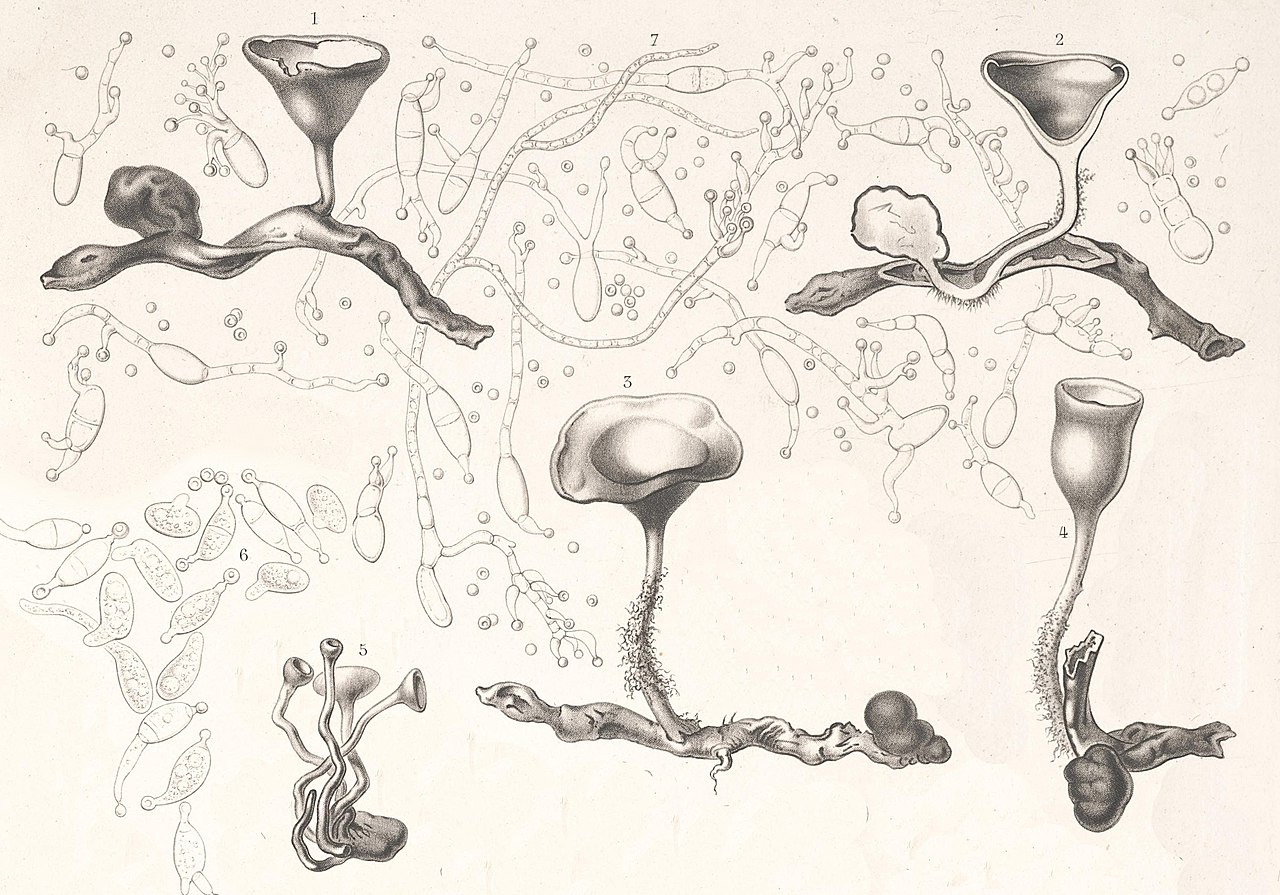
\includegraphics[width=\linewidth]{Figures/PezizaTuberosa.jpg}
    \caption[Illustration of the fungus Dumontinia tuberosa]{Illustration of the fungus Dumontinia tuberosa by physician, mycologist, and illustrator Charles Tulasne (1816–1884) in the book Selecta Fungorum Carpologia (1861–65). (Name of the original work: Peziza tuberosa parasite on Anemone nemorosa)}
    \label{fig:figure-01}
\end{figure}

\section{Side-by-Side Figures}
For the purpose of comparing or for other reasons, you can insert side-by-side figures using both the \verb|\begin{figure}| and \verb|\begin{subfigure}| environments. You can also refer to the sub-figure as \autoref{fig:figure-02.1} and \autoref{fig:figure-02.2}.

\begin{figure}[!htpb]
    \centering
    \begin{subfigure}{0.45\textwidth}
        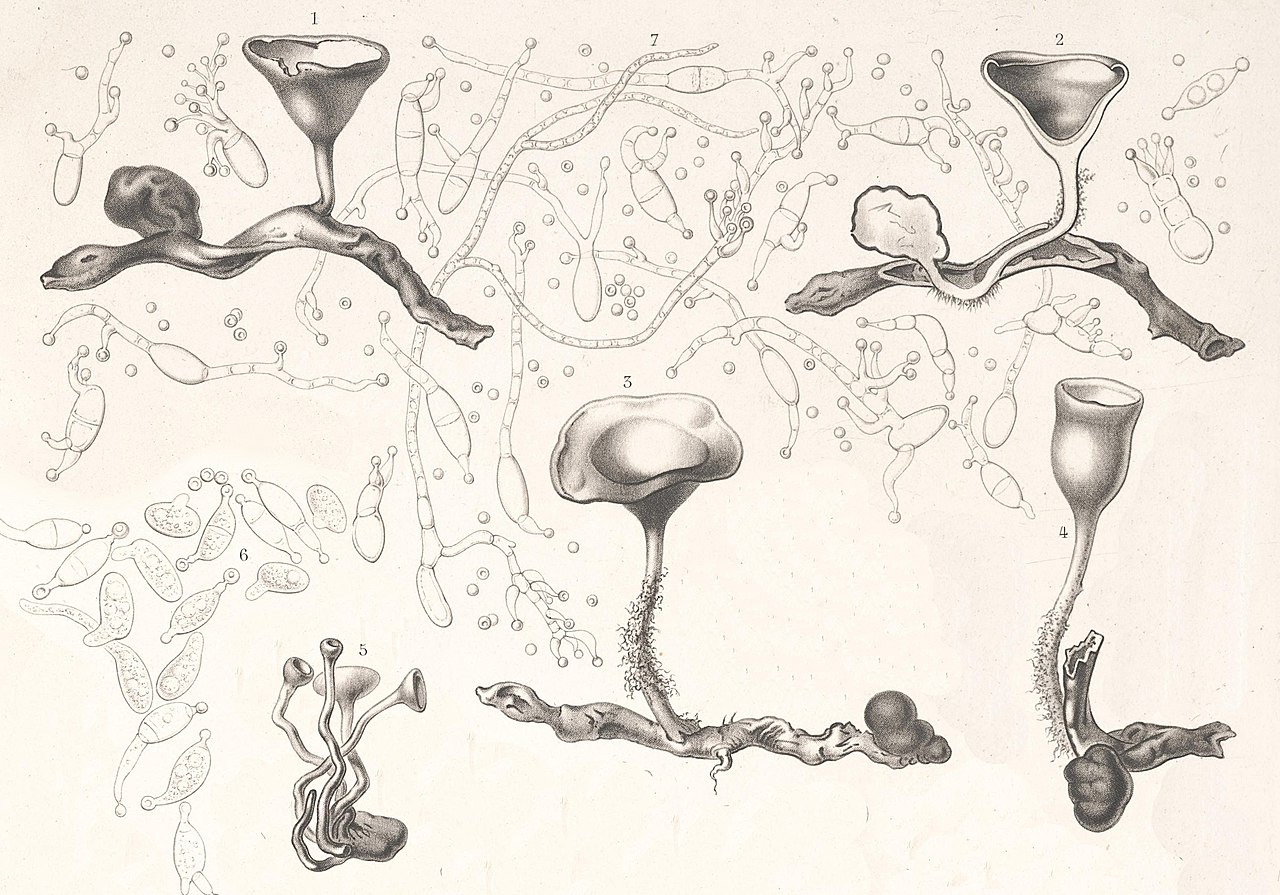
\includegraphics[width=\textwidth]{Figures/PezizaTuberosa.jpg}
        \caption{Caption for Image 1}
        \label{fig:figure-02.1}
    \end{subfigure}
    \hspace{.5cm} % Adjust the space as needed
    \begin{subfigure}{0.45\textwidth}
        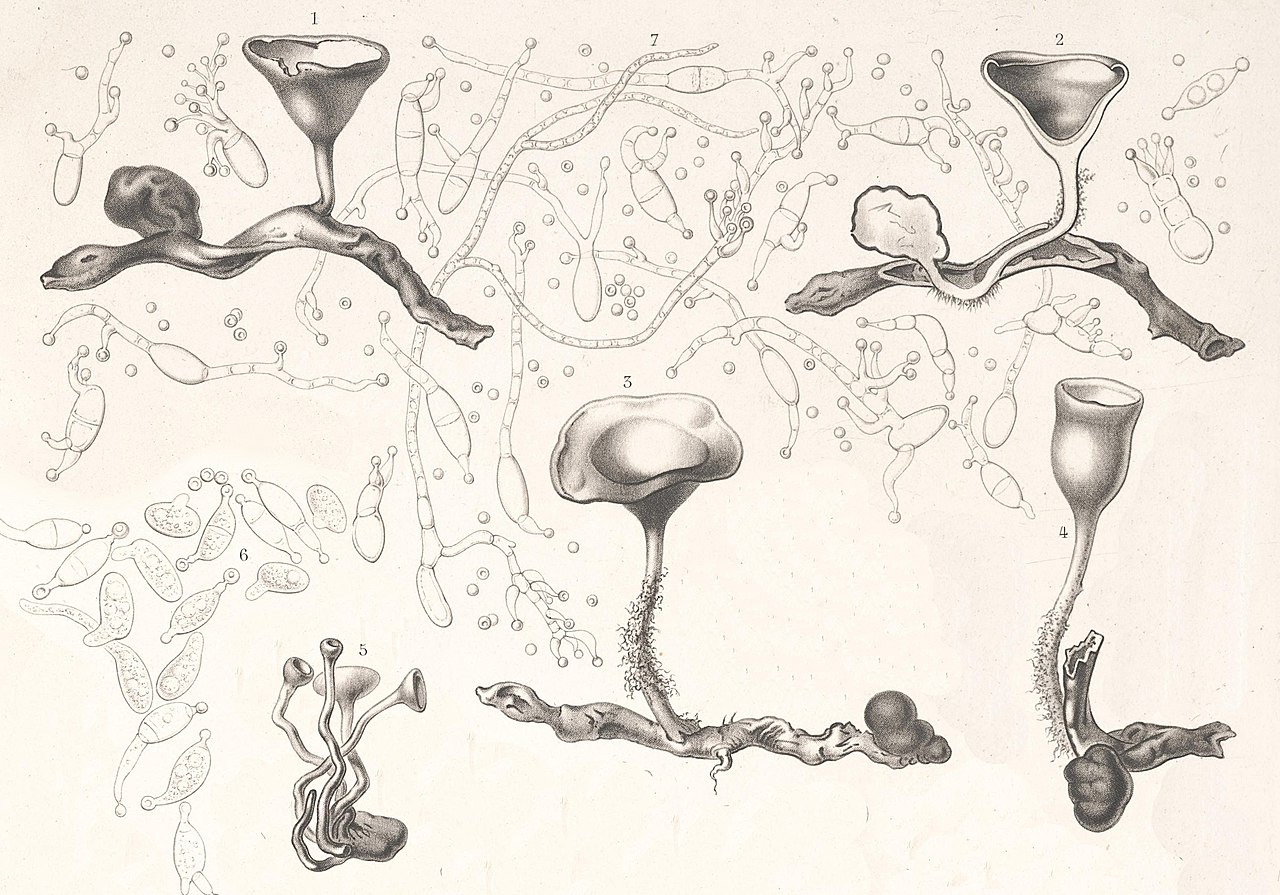
\includegraphics[width=\textwidth]{Figures/PezizaTuberosa.jpg}
        \caption{Caption for Image 2}
        \label{fig:figure-02.2}
    \end{subfigure}
    \caption{Overall Caption for the Figure}
    \label{fig:figure-02}
\end{figure}

To customise the spacing between sub-figures, utilise the \verb|\hspace{VALUE}| command. Establishing adequate spacing is crucial for enhancing visual appeal and ensuring a reader-friendly experience. Below is a code snippet that represents the \autoref{fig:figure-02} - both label and caption text were omitted.

\begin{verbatim}
\begin{figure}[!htpb]
    \centering
    \begin{subfigure}{0.45\textwidth}
        \includegraphics[width=\textwidth]{FIGURE_PATH}
        \caption{TEXT}
        \label{TEXT}
    \end{subfigure}
    \hspace{.5cm} % Adjust the space as needed
    \begin{subfigure}{0.45\textwidth}
        \includegraphics[width=\textwidth]{FIGURE_PATH}
        \caption{TEXT}
        \label{TEXT}
    \end{subfigure}
    \caption{TEXT}
    \label{TEXT}
\end{figure}
\end{verbatim}
\chapter{Tables}
Tables play a vital role in presenting your findings effectively. In this chapter, we delve into various techniques for conveying information through tables, employing different environments available in this template. Although defining tables in \LaTeX\ may appear complex, using this template makes the process more straightforward.

\begin{importantbox}
    Prior to showcasing the different table environments, it's crucial to note that each one must be enclosed within a \verb|\begin{table}| environment. Additionally, it is recommended to utilise the \verb|[!htpb]| float options for improved document placement. \textbf{This advice should be taken into consideration when positioning figures as well}.
\end{importantbox}

\section{Tabular Environment}
The conventional \verb|\begin{tabular}| environment enables you to create a simple yet elegant table. \autoref{tab:table-01} is generated using a centering environment for added emphasis. It also incorporates the \verb|booktab| configuration for a more sophisticated table style.

\begin{table}[!htpb]
    \caption{A Table Showcasing the Usage of the Tabular Environment.}
    \label{tab:table-01}
    \centering
    \begin{tabular}{llc}
        \toprule
        Header 01 & Header 02 & Header 03 \\ 
        \midrule
        Lorem Ipsum & Lorem Ipsum & $\checkmark$ \\
        Lorem Ipsum & Lorem Ipsum & $\checkmark$ \\
        Lorem Ipsum & Lorem Ipsum & - \\
        Lorem Ipsum & Lorem Ipsum & - \\
        Lorem Ipsum & Lorem Ipsum & $\checkmark$ \\
        \bottomrule
    \end{tabular}
\end{table}

\section{Tabularx Environment}
Employ the \verb|\begin{tabularx}| package to construct a table featuring automatically expanding multi-columns. To achieve this automatic behaviour for multi-columns, utilise the following environment: \verb|\begin{tabularx}{\textwidth}{@{}lX@{}}|. Take note that we substitute \verb|X| in place of \verb|l| or \verb|c|, explicitly indicating that the column will function as a multi-column, occupying the entire available space. \autoref{tab:table-02} showcases the usage of the \verb|begin{tabularx}| environment.

\begin{table}[!htpb]
    \caption{A Table Showcasing the Usage of the Tabularx Environment}
    \label{tab:table-02}
    \begin{tabularx}{\textwidth}{@{}lX@{}}
        \toprule
        Header 01 & Header 02 \\ 
        \midrule
        Foo Bar Baz & Quisque cursus, metus vitae pharetra auctor, sem massa mattis sem, at interdum magna augue eget diam. \\
        Ipsum Dolor & Vestibulum ante ipsum primis in faucibus orci luctus et ultrices posuere cubilia Curae; Curabitur aliquet quam id dui. \\
        Dolor Sit & Phasellus condimentum elementum justo, quis interdum est sagittis ac. Vestibulum non arcu sit amet justo lobortis semper. \\
        Amet Consectetuer & Integer nec odio praesent libero sed cursus ante dapibus diam sed nisi vestibulum non arcu. \\
        Consectetuer Adipiscing & Nulla quis sem at nibh elementum imperdiet. Duis sagittis ipsum. Praesent mauris. \\
        \bottomrule
    \end{tabularx}
\end{table}

\section{Longtable Environment}
At times, when dealing with exceptionally lengthy tables, it becomes necessary to split them across multiple pages. In \LaTeX, this can be achieved using the \verb|\begin{longtable}| environment. Feel free to consult \autoref{tab:table-03} for a detailed demonstration of how the \verb|longtable| operates.

\begin{longtable}[c]{llll}
\caption{A Table Showcasing the Usage of the Longtable Environment}
\label{tab:table-03} \\
\toprule
Names & E-Mails & Job/Role \\ \midrule
\endfirsthead
%
\multicolumn{4}{c}%
{{\bfseries Table \thetable\ continued from previous page}} \\
\toprule
Names & E-Mails & Job/Role \\ \midrule
\endhead
%
\bottomrule
\endfoot
%
\endlastfoot
%
Alice Johnson & alice.johnson@email.com & Project Manager \\
Bob Thompson & bob.thompson@email.com & Data Analyst \\
Charlie Davis & charlie.davis@email.com & Marketing Specialist \\
David Miller & david.miller@email.com & QA Tester \\
Emily White & emily.white@email.com & Graphic Designer \\
Frank Martin & frank.martin@email.com & HR Coordinator \\
Grace Turner & grace.turner@email.com & Financial Analyst \\
Henry Lee & henry.lee@email.com & System Administrator \\
Ivy Carter & ivy.carter@email.com & Customer Support \\
Jack Wilson & jack.wilson@email.com & Frontend Developer \\
Jane Reed & jane.reed@email.com & UX Designer \\
Kevin Evans & kevin.evans@email.com & Product Manager \\
Linda Adams & linda.adams@email.com & Accountant \\
Mike Hill & mike.hill@email.com & Network Engineer \\
Nina Garcia & nina.garcia@email.com & Business Analyst \\
Oliver Smith & oliver.smith@email.com & Sales Representative \\
Pamela Turner & pamela.turner@email.com & Legal Counsel \\
Quincy Brown & quincy.brown@email.com & IT Consultant \\
Rachel Moore & rachel.moore@email.com & Content Writer \\
Samuel White & samuel.white@email.com & Research Scientist \\ \bottomrule
\end{longtable}

\section{Complex Tables}
Creating intricate tables in \LaTeX\ can be a somewhat challenging task. Therefore, we highly recommend using the \href{https://www.tablesgenerator.com/}{Table Generator}. With this tool, you can design your table with the desired style and then easily copy and paste it into your document. This approach simplifies the process and helps ensure the accurate representation of complex tables in your \LaTeX\ document. However, it's crucial to keep in mind that a table should be easily comprehensible for the reader and should not be overly complex. The complexity of a table may impede understanding. For example, \autoref{tab:table-04} presents a table with intricate details.

\begin{table}[!htpb]
    \caption{A Table Showcasing the Usage of the Complex Tables}
    \label{tab:table-04}
    \centering
    \begin{tabular}{lcc}
        \toprule
        \multirow{2}{*}{Category} & \multicolumn{2}{c}{\textbf{Details}} \\
        \cmidrule(lr){2-3}
        & Subcategory & Carried Out \\
        \midrule
        \multirow{3}{*}{Long Category Name A} & Long Subcategory Name A & $\checkmark$ \\
        & Ipsum & $\checkmark$ \\
        & Adipiscing & - \\
        \midrule
        \multirow{3}{*}{Long Category Name B} & Long Subcategory Name B & - \\
        & Ipsum & - \\
        & Adipiscing & - \\
        \midrule
        \multirow{3}{*}{Long Category Name C} & Long Subcategory Name C & $\checkmark$ \\
        & Consectetur & $\checkmark$ \\
        & Adipiscing & - \\
        \bottomrule
    \end{tabular}
\end{table}
\chapter{Lists}
Creating lists in \LaTeX\ is straightforward, offering various options to suit your needs. You can generate a bullet list using \verb|\begin{itemize}|, or opt for a numbered list with \verb|\begin{enumerate}|. Below is an example with the \verb|\begin{itemize}| environment.

\begin{itemize}
  \item List entries start with the \verb|\item| command.
  \item Individual entries are indicated with a black dot, a so-called bullet.
  \item The text in the entries may be of any length.
\end{itemize}

As mentioned earlier, you can generate a numbered list using the \verb|\begin{enumerate}| environment. Here is an example:

\begin{enumerate}
  \item Items are numbered automatically.
  \item The numbers start at 1 with each use of the \verb|enumerate| environment.
  \item Another entry in the list.
\end{enumerate}

You can also nest list entries by creating a list inside another list of the same type. Here is an example:

\begin{enumerate}
    \item First level item
    \item First level item
    \begin{enumerate}
        \item Second level item
        \item Second level item
    \begin{enumerate}
        \item Third level item
        \item Third level item
    \begin{enumerate}
        \item Fourth level item
        \item Fourth level item
    \end{enumerate}
    \end{enumerate}
    \end{enumerate}
\end{enumerate}

\begin{importantbox}
    Please note that the labels change automatically regardless of the environment being the same for every list. \textbf{This demonstrates that there's no need to worry about changing the environment for something different.} However, if desired, you have the flexibility to do so.
\end{importantbox}

You can also modify the label of your list to something entirely different that suits your needs. To accomplish this, insert a new \verb|\item| and enclose your desired label in square brackets. For example, \verb|\item[!]| will result in an exclamation point as your new label. Below are some examples of modified labels.

\begin{itemize}
  \item This is my first point
  \item Another point I want to make 
  \item[!] A point to exclaim something!
  \item[$\blacksquare$] Make the point fair and square.
  \item[] A blank label?
\end{itemize}

Finally, you can create a description list. Unlike having a bullet point or a numbered label, a description list enables you to use custom descriptions that suit your list. In the example below, there are three \verb|\item| entries: one without a label, and two with descriptions.

\begin{description}
    \item[Item 1:] This is the first item with a description.
    \item[Item 2:] Another item with a different description.
    \item An item without a specific label.
\end{description}
\chapter{Code Listings}
At times, you may want to include source code from your programs and applications within your document. To achieve this, you can use two nested environments: \verb|\begin{listing}| to create a listing with both caption and label, and \verb|\begin{minted}| for code highlighting. \autoref{listing:c-code} provides an example of a source code in C.

\begin{listing}[!htpb]
\begin{minted}{c}
#include <stdio.h>
int main() {
   printf("Hello, World!"); /*printf() outputs the quoted string*/
   return 0;
}
\end{minted}
\caption{Hello World in C}
\label{listing:c-code}
\end{listing}

The code mentioned above was inserted into the document. However, an alternative approach is to input your code from an external file. To do so, you just need to use the command \verb|\inputminted{CODE_LANGUAGE}{FILE}|. Of course, you should place that command inside of the \verb|\begin{listing}| environment. \autoref{listing:octave-code} illustrates an example of Octave source code that has been input from an external file.

\begin{listing}[!htpb]
\inputminted{octave}{Code/BitXorMatrix.m}
\caption{XOR Operation in Octave}
\label{listing:octave-code}
\end{listing}

In some cases, when you simply want to highlight a specific command, it's recommended not to use \verb|listing| or \verb|minted|. Instead, you should utilise the \verb|\verb| command for inline highlighting or the \verb|\begin{verbatim}| environment for longer sections of highlighted code. An example of a lengthy \verb|verbatim| section is provided below, demonstrating how to create a \verb|listing| with an input code:

\begin{verbatim}
\begin{listing}[!htpb]
    \inputminted{CODE_LANGUAGE}{FILE}
    \caption{TEXT}
    \label{TEXT}
\end{listing}
\end{verbatim}

Sometimes it is necessary to display longer code that occupies more than one page. For this purpose, please use the environment \verb|\begin{longlisting}|. This environment will easily break your code into multiple pages for better readability without you worrying about the size of your code. An example is shown below in \autoref{listing:cobol-code}.

\begin{longlisting}
\begin{minted}{cobol}
IDENTIFICATION DIVISION.
PROGRAM-ID. BankingSystem.

DATA DIVISION.
WORKING-STORAGE SECTION.
01 CUSTOMER-RECORD.
   05 CUSTOMER-NAME       PIC X(30).
   05 CUSTOMER-AGE        PIC 99.
   05 CUSTOMER-BALANCE    PIC 9(7)V99.
   05 CUSTOMER-STATUS     PIC X(10).

01 CUSTOMER-COUNT         PIC 9999 VALUE 0.

01 TEMP-VARIABLES.
   05 TEMP-NAME            PIC X(30).
   05 TEMP-AGE             PIC 99.
   05 TEMP-BALANCE         PIC 9(7)V99.
   05 TEMP-STATUS          PIC X(10).

PROCEDURE DIVISION.

    -- Accept customer details from the console
    ACCEPT CUSTOMER-RECORD FROM CONSOLE.
    ADD 1 TO CUSTOMER-COUNT.

    -- Process customer records until 'EXIT' is entered
    PERFORM PROCESS-CUSTOMER-RECORD UNTIL CUSTOMER-NAME = 'EXIT'.

    -- Display total number of customers processed
    DISPLAY 'Total number of customers: ' CUSTOMER-COUNT.

    -- End the program
    STOP RUN.

PROCESS-CUSTOMER-RECORD.
    -- Copy customer details to temporary variables
    MOVE CUSTOMER-NAME TO TEMP-NAME.
    MOVE CUSTOMER-AGE TO TEMP-AGE.
    MOVE CUSTOMER-BALANCE TO TEMP-BALANCE.
    MOVE CUSTOMER-STATUS TO TEMP-STATUS.

    -- Display customer details
    DISPLAY 'Name: ' TEMP-NAME.
    DISPLAY 'Age: ' TEMP-AGE.
    DISPLAY 'Balance: ' TEMP-BALANCE.
    DISPLAY 'Status: ' TEMP-STATUS.

    -- Accept next customer record
    ACCEPT CUSTOMER-RECORD FROM CONSOLE.
    ADD 1 TO CUSTOMER-COUNT.
END PROGRAM BankingSystem.
\end{minted}
\caption{COBOL Code for a Basic Banking System}
\label{listing:cobol-code}
\end{longlisting}


\chapter{Conclusion}
\blindtext

% Bibliography
\blankpage\printbibliography

\appendix
% Annexes:
\ifthenelse{\equal{\getLanguage}{portuguese}}{%
    \addtocontents{toc}{\protect\contentsline{chapter}{Anexos}{}{}}
}{%
    \addtocontents{toc}{\protect\contentsline{chapter}{Annexes}{}{}}
}

\setcounter{chapter}{12} % To start at the "M" chapter
\blankpage\newgeometry{margin=4cm}
\begin{center}
    \fontfamily{ppl}\selectfont % Font family
    \scshape % Font style
    \thispagestyle{empty}
        
    \vspace*{\fill}
    \ifthenelse{\equal{\getLanguage}{portuguese}}{%
        {\LARGE\textcolor{redreport}{Anexos}\par}
    }{%
        {\LARGE\textcolor{redreport}{Annexes}\par}
    }
    \vspace*{\fill}
\end{center}
\restoregeometry\blankpage
\chapter{Annex A}
\blindtext
\begin{landscapemode}{297mm}{420mm} % These are the recommended dimensions for a landscape layout. Adjust to your own preference.
	\chapter{Annex B}
	\blindtext[5]
\end{landscapemode}


% Back Page
\ifthenelse{\equal{\getLanguage}{portuguese}}{%
    \pdfbookmark[0]{Contra Capa}{contracapa} % Add entry to PDF
}{%
    \pdfbookmark[0]{Back Page}{backpage} % Add entry to PDF
}

\blankpage\newgeometry{margin=4cm}
\fontfamily{ppl}\selectfont % Font family
\scshape % Font style
\small
\thispagestyle{empty}
    
\vspace*{\fill}
\begin{flushright}
    \begin{minipage}{0.5\linewidth}
        \begin{flushright}
            \textcolor{redreport}{\univname}
        
            \vspace{1.5\baselineskip}
        
            % https://tex.stackexchange.com/questions/10130/use-the-values-of-title-author-and-date-on-a-custom-title-page
            \makeatletter{\@title}\makeatother
    
            \vspace{1.5\baselineskip}
    
            \textcolor{redreport}{\firstauthorname} \\
            \textit{\studentnumberprefix\firstauthornum}
            \vspace{0.5\baselineskip}
    
            \ifdefined\secondauthorname
                \textcolor{redreport}{\secondauthorname} \\
                \textit{\studentnumberprefix\secondauthornum}
                \vspace{0.5\baselineskip}
            \fi
    
            \ifdefined\thirdauthorname
                \textcolor{redreport}{\thirdauthorname} \\
                \textit{\studentnumberprefix\thirdauthornum}
                \vspace{0.5\baselineskip}
            \fi
    
            \vspace{1.5\baselineskip}
            
            {\thedate}
        \end{flushright}
    \end{minipage}
\end{flushright}
\restoregeometry

\end{document}
